\subsection{Implementacja}
W mojej pracy zdecydowałem się na skorzystanie z platformy Azure~\ref{MS_AzureSection} - 
wpłynęły na nią przyjazny interfejs, łatwość instalacji agenta, jasna struktura tworzenia pipeline'ów 
oraz mnogość instrukcji i poradników dotępnych w Internecie.

Na przykładzie aplikacji Navigator~\ref{NavigatorAppSection} chciałbym przedstawić proces \\
planowania i konfiguracji pipeline'a.

\subsubsection{Określenie potrzeb i możliwości}
W moim projekcie, oprócz samej kompilacji, postanowiłem zaimplementować etap testowania 
oraz wydania aplikacji na wspomnianym wcześniej GitHub Releases~\cite{githubReleases}.
Na rysunku \ref{img:JobsOverview} widzimy efekt wykonania takiego pipeline'a z poziomu 
widoku zarządzania pipeline'ami na stronie Microsoft Azure:

\begin{figure}[ht]
    \centering
    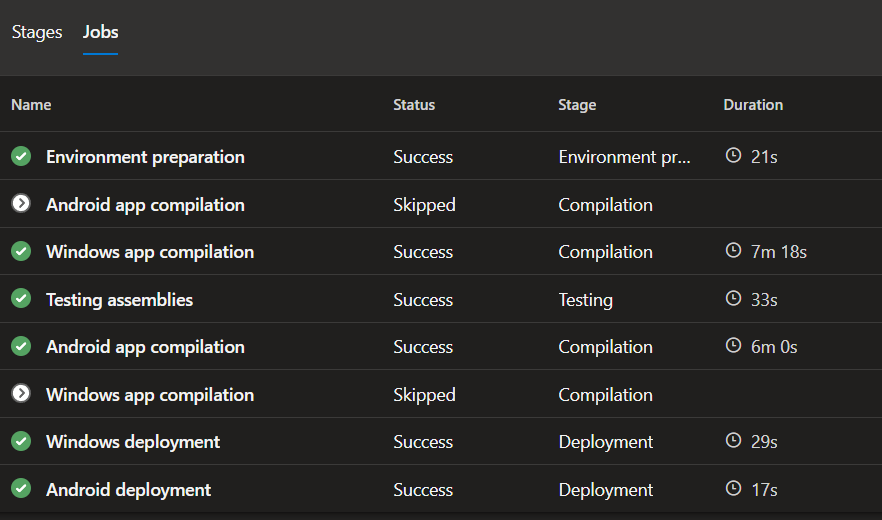
\includegraphics[scale=0.5]{JobsOverview.png}
    \caption{Zadania (ang. Joby) wykonane przez pipeline}
    \label{img:JobsOverview}
\end{figure}

\subsubsection{Przygotowanie środowiska kompilacyjnego}
Pierwszym krokiem było zainstalowanie specjalnego oprogramowania, 
które wykonuje wszystkie kroki zdefiniowane w pipelinie - Azure Build Agent~\footnote[1]{
    \href{https://learn.microsoft.com/en-us/azure/devops/pipelines/agents/agents}{
        Informacje o Agentach
    }
}.
Ze względu na dysponowanie własną, dostępną maszyną zdecydowałem się na tą opcję,
jednak taki sam efekt można osiągnąć opłacając maszyny wirtualne, udostępniane przez Microsoft. \\%
Po krótkiej konfiguracji Agent był gotowy do wykonywania zleconego \\%
pipeline'owego skryptu, ale należało jeszcze dodać zmienne środowiskowe, 
które pozwalają na skorzystanie z określonych funkcji zadań (przykładem jest użycie Javy~\ref{javaTask}).

\subsubsection{Zdefiniowanie wymaganych akcji}
Utworzenie pakietu mojej aplikacji napisanej w .NET MAUI przebiega za pomocą wywołania kompilatora 
\verb|dotnet| z opcją \cprotect{\href{https://learn.microsoft.com/en-us/dotnet/core/tools/dotnet-publish}}{\verb|publish|}, 
która uruchamia przywrócenie wszystkich zależności (\verb|restore|), 
kompiluje ją (\verb|build|) oraz pakuje do przewidzianego w konfiguracji projektu (\verb|.csproj|) formatu~\cprotect\footnote{%
    Interesującym może okazać się fakt, że aplikację w .NET MAUI kompilujemy w oparciu o projekt, a nie rozwiązanie (\verb|.sln|).
    Jest to spowodowane kolejnością interpretacji plików
}.

Zdecydowałem się na podpisywanie aplikacji osobnym zadaniem ze względu na modularność,
jak również ze względu na chęć ominięcia szczegółów tej operacji wewnątrz samego kodu (tj. w pliku projektu).

\subsubsection{Podejście graficzne}
Moja pierwsza próba konfiguracji została podjęta w ramach graficznego konfiguratora, 
który pozwolił mi na wykonanie (jak się później okazało szkicu) mojego pipeline'a.
Na rysunkach~\ref{img:PipelineGuiApproach} i \ref{img:taskGroupMauiPrepare} możemy zobaczyć jego schemat działania:\\
\begin{figure}[ht]
    \centering
    \begin{minipage}[t]{0.48\textwidth}
        \centering
        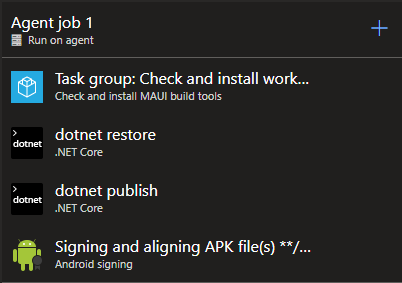
\includegraphics[width=\textwidth]{PipelineGuiApproach.png}
        \caption{Grupa zadań \\%
        inicjujących środowisko \\%
        (szczegóły na rys.~\ref{img:taskGroupMauiPrepare}) oraz \\%
        publikacja i podpisanie cyfrowe}
        \label{img:PipelineGuiApproach}
    \end{minipage}
    \hfill
    \begin{minipage}[t]{0.47\textwidth}
        \centering
        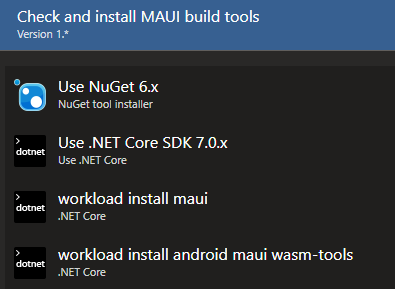
\includegraphics[width=\textwidth]{taskGroupMauiPrepare.png}
        \caption{Zawartość grupy zadań \\inicjujących środowisko}
        \label{img:taskGroupMauiPrepare}
    \end{minipage}
\end{figure}

\newpage

O ile ten pipeline spełniał swoje zadanie na minimalnym poziomie, czyli przygotowywał potrzebne narzędzia 
oraz kompilował i podpisywał aplikację skierowaną na system Android, to jednak jego efektywność i prostota 
utrzymania pozostawiały wiele do życzenia.

Pierwszym z zarzutów jest zbędne wykonanie \verb|dotnet restore| - choć narzut pracy 
jest stosunkowo niewielki, wprowadza kolejny punkt zaczepienia do zadania pytania "czy mogę to zmienić?", 
które mogłaby zadać osoba bliżej niezaznajomiona z działaniem narzędzia.

Drugim problemem okazał się brak wykorzystania zmiennych, które wraz z parametryzacją procesu 
pozwoliłyby na uczynienie go bardziej elastycznym i uniwersalnym. 
Pomimo skorzystania z bezpiecznych zmiennych w procesie podpisywania pliku APK, 
byłem w stanie skorzystać wyłącznie z jednego, wcześniej przygotowanego zestawu danych, 
którego nie mogłem zmienić przed wywołaniem pipeline'a.

% \begin{figure}[hb]
%     \centering
%     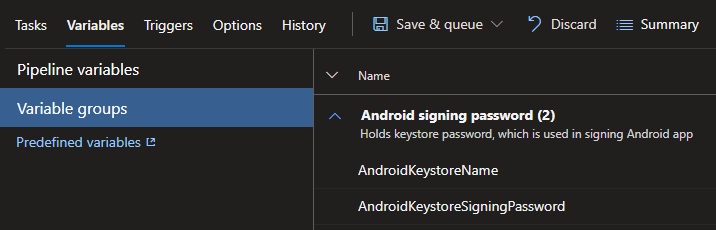
\includegraphics[width=0.75\textwidth]{variableGroups.png}
%     \caption{Predefiniowane zmienne przechowujące nazwę oraz hasło podpisujące certyfikat}
%     \label{img:variableGroups}
% \end{figure}
